%!TEX root = design_doc.tex

\section{User Interface}

As stated in previous sections, our code library integrates sampling, estimation, clustering, and statistical inference for time series models. To support these functionalities, we build interfaces that decompose the whole project into well-organized parts that enables integration.

In specific, our project consists of five classes: ``Model'', ``Simulation'', ``Optimization'', ``Inference", and `` Clustering''. The pivotal idea is to  decouple the times series models and the methods that work on models. By doing so, we can not only obtain  a  clearer view of the whole picture, but, more importantly, enables users to  apply the statistical methods to more datasets, thus enhance  usability. A detailed description of these class are as follows.


The ``Model'' class consists of a variety of  time series models. Each model is identified by its  parameters and the major goal of data analysis is to learn these parameters from the data. For each model, we first define a  function that formulates the model. Then we define a loss function and the goal of learning the model is reduce to minimizing the loss function. Since we use first- and second-order optimization methods, we also compute its gradient and Hessian.

The ``Simulation'' class consists tools to sample data from the time series models. Although working on real-world datasets is more interesting, simulated data enables us to access the performance of the statistical procedures. The sampling function treats a model as input and use Bayesian sampling method such as Markov Chain Monte Carlo  and Gibbs sampling to generate simulated data.

The ``Optimization'' class consists of optimization tools. In general, an optimization procedure minimizes the loss function using gradient and/or Hessian information of the loss function. In this class, we will realize various popular optimization algorithms that enjoy great empirical success in deep learning. Some examples are gradient descent, stochastic gradient descent, momentum method, Adgrad, conjugate gradient, Newton method.

The ``Inference'' class consists of statistical procedures for time series models. We construct confidence intervals and hypothesis tests for the model parameters. After estimating the model, it is not clear whether estimation is accurate. Statistical inference enables us to access the uncertainty of our estimation procedure. Out inference functions will take the model and data as input, and outputs a confidence interval or test statistic. When using the simulated data, statistical inference enables us to quantitively understand the performance of estimation.

Finally, the ``Clustering'' class consists methods to cluster data into groups. For finance data, this task is of great importance. For example, stocks in different sectors behave differently. It is meaningful to cluster these stocks to reveal more fine-grained information of the market. Some of the procedures consists of K-means, Gaussian mixture model, hierarchical clusterin, and DBSCAN algorithm. Note that clustering algorithms work for general datasets. Thus this class may potentially have broader application. 

\begin{figure}[htbp]
\begin{center}
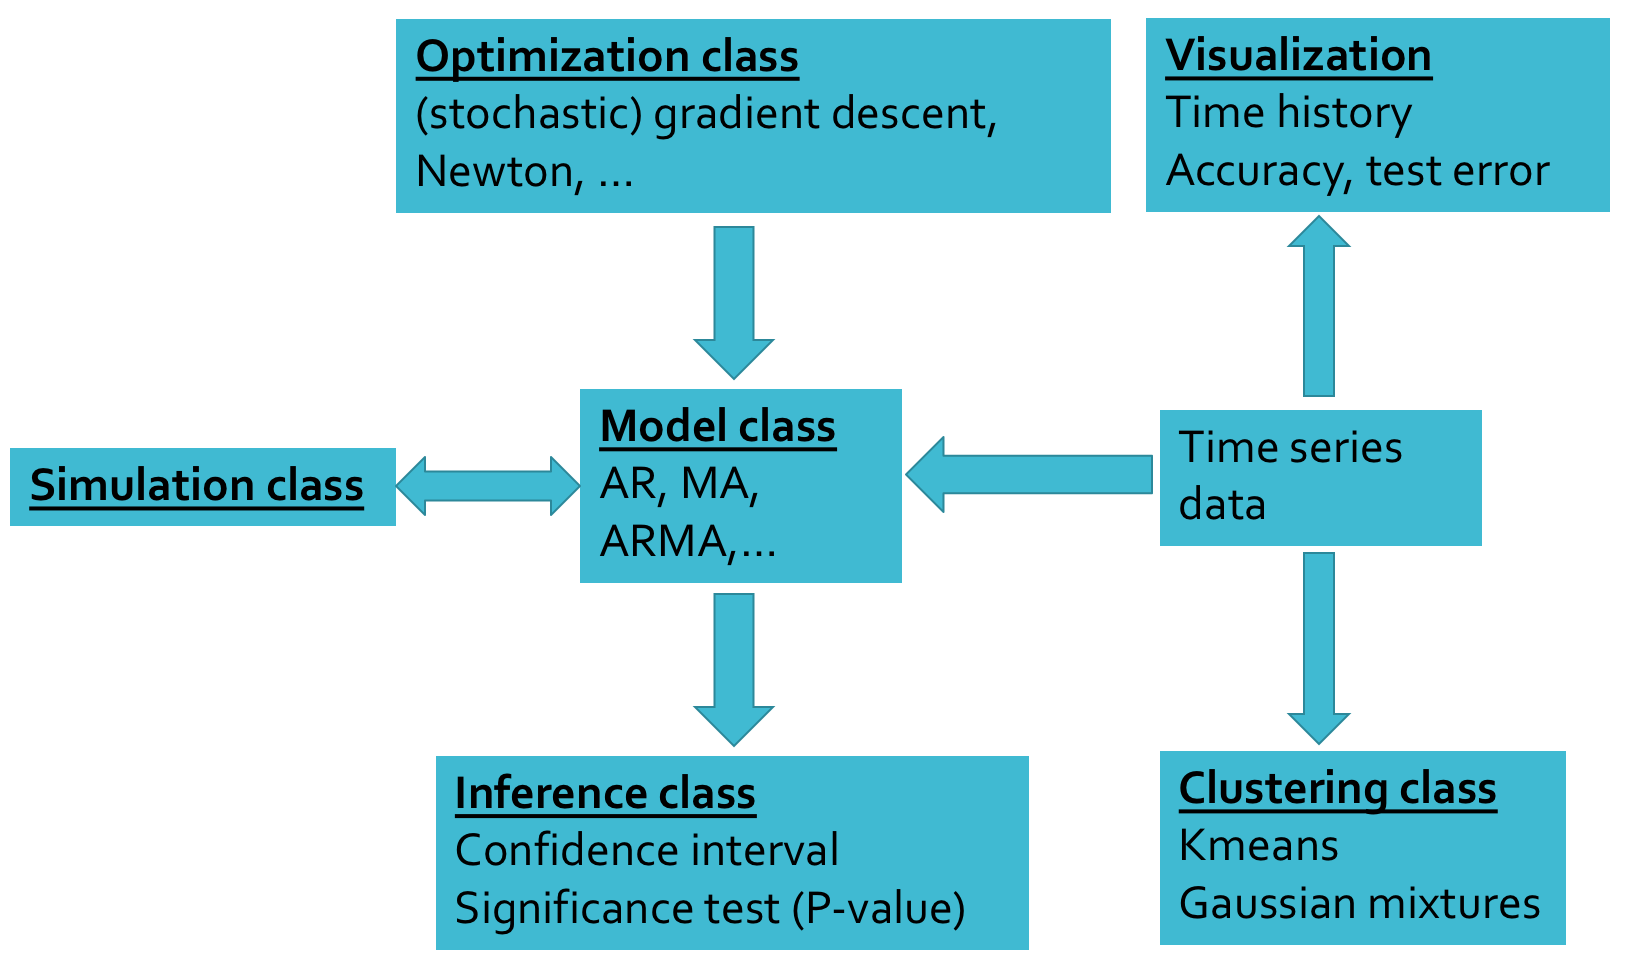
\includegraphics[width = 10cm]{./Figures/flowchart.png}
\caption{The relationship between the five classes of our project}
\label{default}
\end{center}
\end{figure}

